\section{Apstraktna sintaksna stabla - AST}
\label{sec:AST}

Kako bi se od datoteke na fajl sistemu koja sadrži izvorni kod programa 
došlo do izvršivog programa, potrebno je izvršiti više koraka 
\cite{CompilerConstruction}:
\begin{itemize}
    \item pretprocesiranje
    \item prevođenje
    \item asembliranje
    \item linkovanje
\end{itemize}

Ovi koraci će biti opisani na jednom primeru. Pretpostavimo da želimo 
da kompajliramo kod pisan u programskom jeziku C prikazan na slici 
\ref{fig:CompilationProcessInit}. Primetimo da postoji greška u datom
kodu - simbol \texttt{c} koji se koristi u dodeli \texttt{a = a + c} 
će biti prepoznat kao identifikator koji ne odgovara nijednoj 
deklarisanoj promenljivoj - stoga ne možemo prevesti ovaj kod. Ovo, 
doduše, nije sintaksna greška - izraz \texttt{a + c} je sasvim validan 
u programskom jeziku C bez analize konteksta u kom se javlja. Problem 
će postati očigledan tek nakon parsiranja izvornog koda i provere 
ispunjenosti sintaksih pravila. Ovakve greške se nazivaju 
\emph{semantičke greške}.

\begin{figure}[h!]
    \begin{lstlisting}
    #include<stdio.h>

    #define T int

    int main()
    {
        T a, b;
        a = a + c;        // c nije deklarisano
        printf("%d", a);
        return 0;
    }
    \end{lstlisting}
    \caption{Primer izvornog koda pisanog u programskom jeziku C.}
    \label{fig:CompilationProcessInit}
\end{figure}

U fazi pretprocesiranja se vrše samo tekstualne operacije kao što su
brisanje komentara ili zamena makroa u jezicima kao što je C. Prvo 
mesto gde se vrši analiza sadržaja izvornog fajla je faza prevođenja.
Tu analizu vrši program koji se naziva \emph{pretprocesor}. Rezultat 
rada pretprocesora za kod sa slike \ref{fig:CompilationProcessInit} 
bi izgledao kao na slici \ref{fig:CompilationProcessPrep} \footnote{
U nekim implementacijama C standardne biblioteke, moguće je da se 
poziv funckije \texttt{printf} zameni pozivom funkcije \texttt{fprintf}
sa ispisom na \texttt{stdout}. U standardu se propisuje da funkcije 
kao što je \texttt{printf} mogu biti implementirane kao makroi. Izlaz 
na slici \ref{fig:CompilationProcessPrep} je generisan od strane 
\texttt{GCC 7.4.0} po C11 standardu.} i ovo nije slučaj u datom 
okruženju.

\begin{figure}[h!]
    \begin{lstlisting}
    int main()
    {
        int a, b;
        a = a + c;
        printf("%d", a);
        return 0;
    }
    \end{lstlisting}
    \caption{Rezultat rada pretprocesora za kod sa slike 
             \ref{fig:CompilationProcessInit}.}
    \label{fig:CompilationProcessPrep}
\end{figure}

Prilikom faze prevođenja, kako prevodilac ne bi radio nad sirovim 
karakterima izvornog koda, potrebno je izvršiti pripremu istog. 
Prevodilac ima u vidu moguće elemente programskog jezika, tzv. 
\emph{tokene}, koje treba prepoznati u datom fajlu - ključne reči, 
operatore, promenljive itd. Program koji radi \emph{tokenizaciju} -
prepoznavanje tokena u izvornom fajlu - se naziva \emph{lekser}. 
Pojednostavljen primer tokena koje lekser pokušava da prepozna 
se može videti na slici \ref{fig:CLexerExample}. Primer izlaza
leksera za izlaz pretprocesora sa slike \ref{fig:CompilationProcessPrep}
se može videti na slici \ref{fig:CompilationProcessLex} \footnote{Moderni
kompajleri nemaju zapravo odvojene faze u kojima se pozivaju lekser i
parser, već se tokenizacija odvija paralelno sa fazom parsiranja. Međutim, 
to nas ne sprečava da ispišemo tokene svaki put kada ih registrujemo, i 
to je demonstrirano na slici \ref{fig:CompilationProcessLex}.}.

\begin{figure}[h!]
    \begin{lstlisting}[language={}]
    Identifier : IdentifierNondigit 
                 (IdentifierNondigit | Digit)*
               ;

    IdentifierNondigit : Nondigit
                       | UniversalCharacterName
                       ;

    Nondigit : [a-zA-Z_]
             ;

    Digit : [0-9]
          ;
    \end{lstlisting}
    \caption{Primer delimične definicije tokena za ime promenljive po C11 standardu.}
    \label{fig:CLexerExample}
\end{figure}

\begin{figure}[h!]
    \begin{lstlisting}[language={}]
    identifier 'main'	 [LeadingSpace]	Loc=<sample.c:3:5>
    l_paren '('		Loc=<sample.c:3:9>
    r_paren ')'		Loc=<sample.c:3:10>
    l_brace '{'	 [StartOfLine]	Loc=<sample.c:4:1>
    int 'int'	 [StartOfLine] [LeadingSpace]	Loc=<sample.c:5:5>
    identifier 'a'	 [LeadingSpace]	Loc=<sample.c:5:9>
    comma ','		Loc=<sample.c:5:10>
    identifier 'b'	 [LeadingSpace]	Loc=<sample.c:5:12>
    semi ';'		Loc=<sample.c:5:13>
    identifier 'a'	 [StartOfLine] [LeadingSpace]	Loc=<sample.c:6:5>
    equal '='	 [LeadingSpace]	Loc=<sample.c:6:7>
    identifier 'a'	 [LeadingSpace]	Loc=<sample.c:6:9>
    plus '+'	 [LeadingSpace]	Loc=<sample.c:6:11>
    identifier 'c'	 [LeadingSpace]	Loc=<sample.c:6:13>
    semi ';'		Loc=<sample.c:6:14>
    identifier 'printf'	 [StartOfLine] [LeadingSpace]	Loc=<sample.c:7:5>
    l_paren '('		Loc=<sample.c:7:11>
    string_literal '"%d"'		Loc=<sample.c:7:12>
    comma ','		Loc=<sample.c:7:16>
    identifier 'a'	 [LeadingSpace]	Loc=<sample.c:7:18>
    r_paren ')'		Loc=<sample.c:7:19>
    semi ';'		Loc=<sample.c:7:20>
    return 'return'	 [StartOfLine] [LeadingSpace]	Loc=<sample.c:8:5>
    numeric_constant '0'	 [LeadingSpace]	Loc=<sample.c:8:12>
    semi ';'		Loc=<sample.c:8:13>
    r_brace '}'	 [StartOfLine]	Loc=<sample.c:9:1>
    eof ''		Loc=<sample.c:9:2>
    \end{lstlisting}
    \caption{Proces tokenizacije koda pisanog po C11 gramatici. Generisano
    uz pomoć \texttt{clang} \cite{Clang} kompajlera.}
    \label{fig:CompilationProcessLex}
\end{figure}

Nakon završetka rada leksera potrebno je parsirati dobijene tokene.
Parsiranje vrši program koji se naziva \emph{parser}. Parser, slično
kao što lekser ima definicije tokena jezika, mora imati informacije 
o gramatici jezika. Gramatika programskog jezika se najčešće definiše
putem kontekstno-slobodnih gramatika \cite{ContextFreeGrammars}, 
čiji je primer dat na slici \ref{fig:CompilationProcessGram}.

\begin{figure}[h!]
    \begin{lstlisting}[language={}]
    functionDefinition
        :   declarationSpecifiers? declarator declarationList? compoundStatement
        ;

    declarationList
        :   declaration
        |   declarationList declaration
        ;

    declaration
        :   declarationSpecifiers initDeclaratorList ';'
        | 	declarationSpecifiers ';'
        |   staticAssertDeclaration
        ;
    \end{lstlisting}
    \caption{Isečak gramatike programskog jezika C po standardu C11.}
    \label{fig:CompilationProcessGram}
\end{figure}

Izlaz rada parsera je \emph{stablo parsiranja} (eng. \emph{parse tree} 
ili \emph{derivation tree}). Takvo stablo i dalje sadrži sve relevantne
informacije o izvornom kodu. Vizuelni prikaz rada parsera za gramatiku
sa slike C11 i izvonog koda sa slike \ref{fig:CompilationProcessPrep} je
dat na slici \ref{fig:CompilationProcessPars}. Stablo parsiranja se 
koristi u narednim fazama prevođenja.

\begin{figure}[h!]
    \centering
    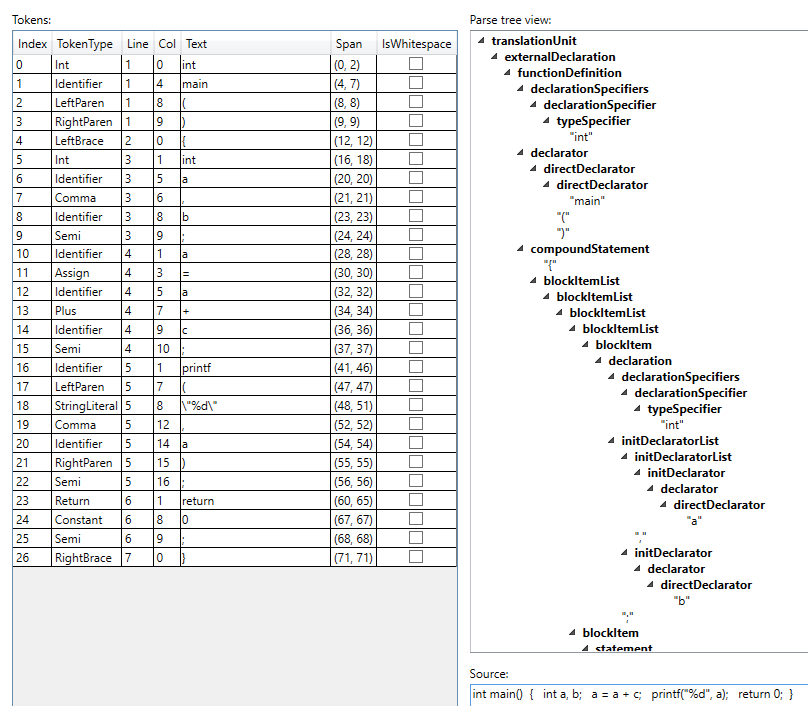
\includegraphics[scale=0.5]{images/parse_tree.png}
    \caption{Prikaz stabla parsiranja koje generiše parser kreiran od strane 
    alata ANTLR4 za C11 gramatiku. Vizualizacija prikazana pomoću dodatka 
    za Visual Studio: \url{https://github.com/zspitz/ANTLR4ParseTreeVisualizer}}
    \label{fig:CompilationProcessPars}
\end{figure}

Za potrebe ovog rada, što se kompilacionog procesa tiče, dovoljno je 
pozvnavanje navedenog. Stoga neće biti reči o daljim koracima u fazi 
prevođenja (semantička provera i sl.) niti o fazama asembliranja i 
linkovanja. Zainteresovani čitalac može više detalja pronaći u 
\cite{CompilerConstruction}. 

Stablo parsiranja sadrži sve informacije potrebne u fazi parsiranja
uključujući detalje koje samo parser koristi. Sa druge strane, 
apstraktno sintaksno stablo sadrži samo sintaksnu strukturu u 
jednostavnijoj formi. Na slici \ref{fig:CompilationProcessPars1} se
može videti koliko je stablo parsiranja komplikovano čak i za naizgled
jednostavne aritmetičke izraze. Razlog ovolike komplikovanosti dolazi 
iz rekurzivnih pravila definisanih u C11 gramatici. Parseru su sve
ove informacije potrebne ali na apstratknijem nivou nisu potrebne.
Jedina važna odlika izraza \texttt{a + c} je ta da je to zbir 
vrednosti nekih promenljivih. Sve ostale informacije su nepotrebne.
Na slici \ref{fig:ASTSimple} možemo videti različita apstraktna 
sintaksna stabla za pomenuti izraz, ali takođe i za malo 
komplikovanije izraze. Podrazumeva se, naravno, da je ulaz već 
tokenizovan. 

\begin{figure}[h!]
    \centering
    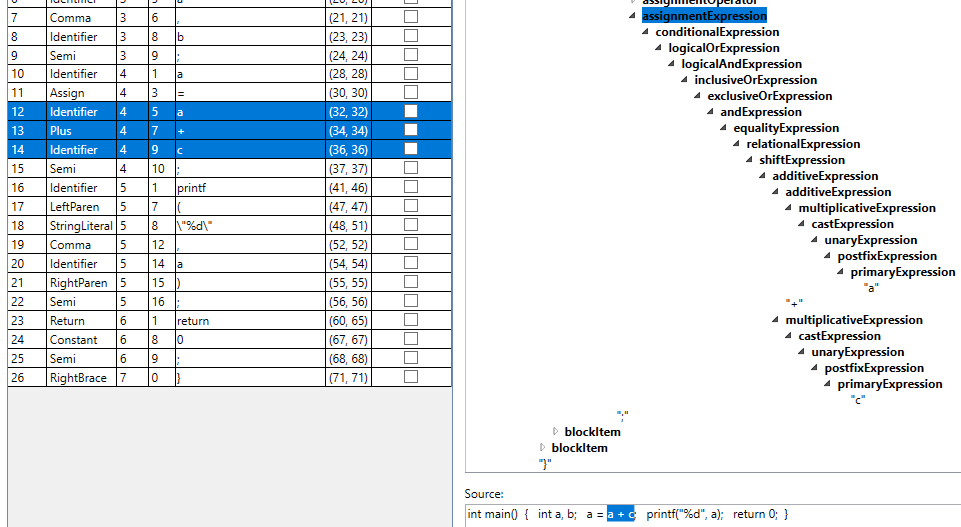
\includegraphics[scale=0.45]{images/parse_tree_expr.png}
    \caption{Prikaz kompleksnosti stabla parsiranja za izraz 
    \texttt{a + c} u C11 gramatici. Vizualizacija prikazana pomoću 
    dodatka za Visual Studio: 
    \url{https://github.com/zspitz/ANTLR4ParseTreeVisualizer}} 
    \label{fig:CompilationProcessPars1}
\end{figure}

\begin{figure}[h!]
    \centering
    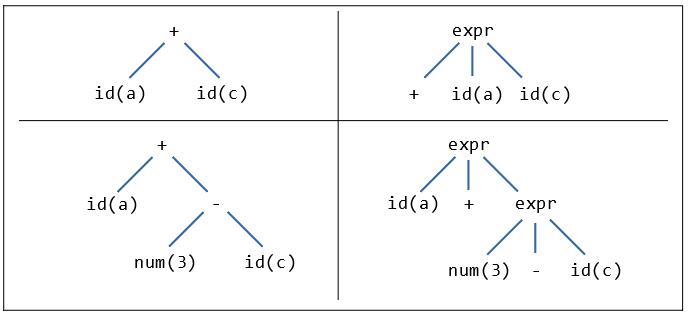
\includegraphics[scale=0.8]{images/ast.png}
    \caption{Varijante apstraktnih sintaksnih stabala bez regularnosti
    (levo) i sa regularnošću (desno) za izraze \texttt{a + c} (gore) i 
    \texttt{a + (3 - c)} (dole).} 
    \label{fig:ASTSimple}
\end{figure}

Uloga apstraktnih sintaksnih stabala je da pokažu semantiku strukture
koda preko stabala. Kao što se vidi na slici \ref{fig:ASTSimple}, 
postoji određeni nivo slobode u dizajniranju ovih stabala. Generalno,
\emph{terminalni simboli}, simboli koji predstavljaju listove stabla
parsera, koji odgovaraju operatorima i naredbama se podižu naviše i 
postaju koreni podstabala, dok se njihovi operandi ostavljaju kao 
njihovi potomci u stablu. Desna stabla sa slike ne prate u potpunosti
ovaj princip, ali se takođe koriste zbog regularnosti izraza - recimo
ukoliko binarni izraz posmatramo kao koncept, mnogo je lakše raditi
sa ovakvom strukturom. Ovakva struktura će biti korišćena u dalje u 
implementaciji programa. Primetimo takođe da se u stablima za izraz 
\texttt{a + (3 - c)} (dole) implicitno sačuvala informacija o 
prioritetu operacije oduzimanja u izrazu. Jasno je, dakle, da se 
računanje vrednosti aritmetičkih izraza onda vrši kretanjem od 
listova stabla ka korenu.

Može se primetiti da su apstraktna sintaksna stabla 
zapravo apstrakcija stabla parsiranja, jer više istih izraza jezika 
može imati isto apstraktno sintaksno stablo ali različito stablo
parsiranja; na primer, ako razmatramo izraz \texttt{(a + 5) - x / 2} 
i izraz \texttt{a + 5 - (x / 2)}.

Apstrakna sintaksna stabla će u daljem tekstu biti referisana 
skraćenicom \emph{AST}, koja dolazi od engleskog naziva za ova stabla
- \emph{Abstract Syntax Trees}. Takođe, reči samom dizajnu i tipovima 
čvorova AST-ova korišćenih u implementaciji će biti u poglavlju 
\ref{TODO}. U narednom poglavlju će više biti reči o alatu koji je 
korišćen za kreiranje parsera za C11 gramatiku (ali i za proizvoljne
gramatike), koji daje mogućnost jednostavnog obilaska istog i pruža
intuitivan način za izvršavanje logike nad stablom parsiranja, što
uključuje i izradu AST-a apstrakcije.
